\documentclass{article}
\usepackage[utf8]{inputenc}
\usepackage{graphicx}

\title{Image Processing : Assignment-1}
\author{Digdarshan Kunwar, Eaindra Wun Pyae}
\date{February 2021}

\begin{document}

\maketitle

\section{Erosion}
\subsection{Erosion of f1 by square of size 3}

Considering the center of the SE (3 $\times$ 3) as the origin (0,0), a padding of 1 is added to all borders of f1 as indicated below as 'img\_with\_boundary'. Since f1 is saved in the binary format, we have to check whether all 8 neighbors of each pixel of 'img\_with\_boundary' are identical to 8 neighbors of the origin in the SE. We start from (0,0) of 'img\_with\_boundary', and shift in column-wise, and row-wise if we have reached the rightmost column of the borderd image. The final result is as shown in 'image after operation' of Figure \ref{fig:ef1_e1}. \\
\begin{figure}[h!]
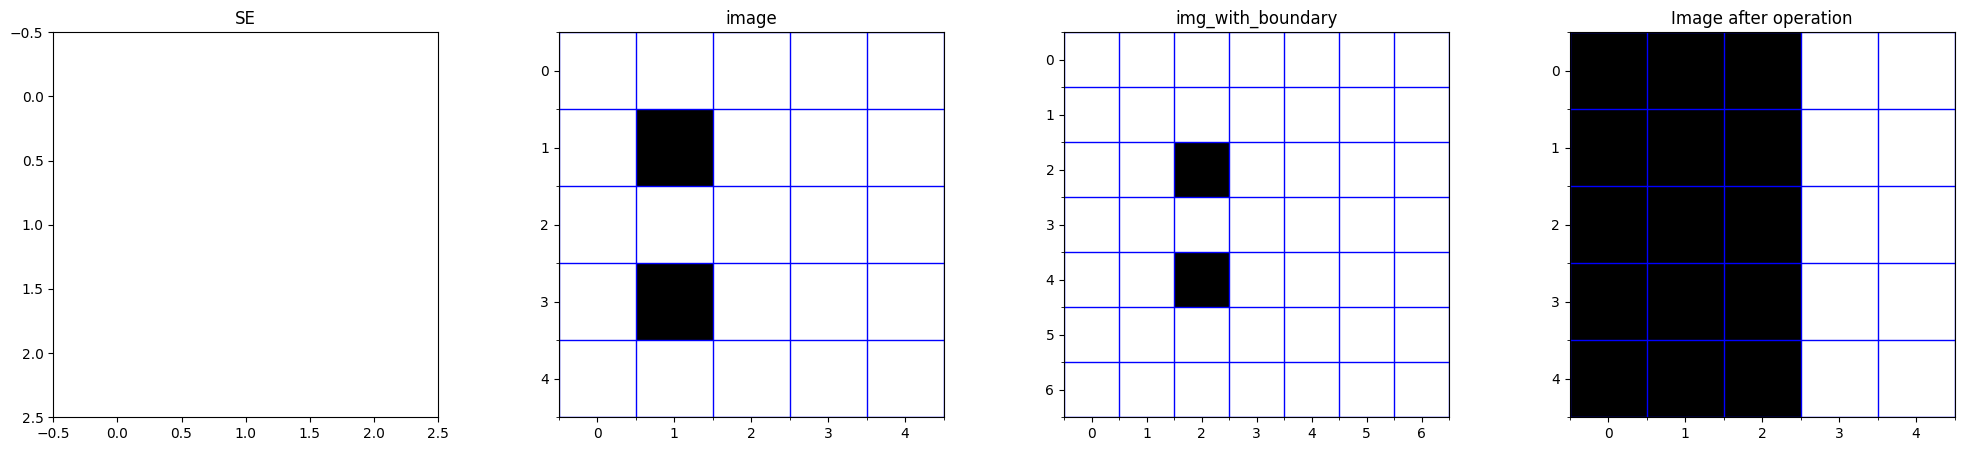
\includegraphics[width=\linewidth]{images/ef1_e1.png}
\caption{Erosion of f1 by square of size 3}
\label{fig:ef1_e1}
\end{figure}
\\ 

\subsection{Erosion of f2 by vertical line of length 3 }
 The center of the SE would be the middle pixel since the given SE is a vertical line. The top and bottom border paddings of size 1 with the maximum value inside f2 (i.e. 5) are applied as indicated below as 'img\_with\_boundary'. During the erosion of a gray-scale image, each pixel is replaced with the minimum pixel value in the neighborhood which are overlapped with the SE in each iteration. The final result is as shown in 'image after operation' of Figure \ref{fig:ef2_e2}. \\
\begin{figure}[h!]
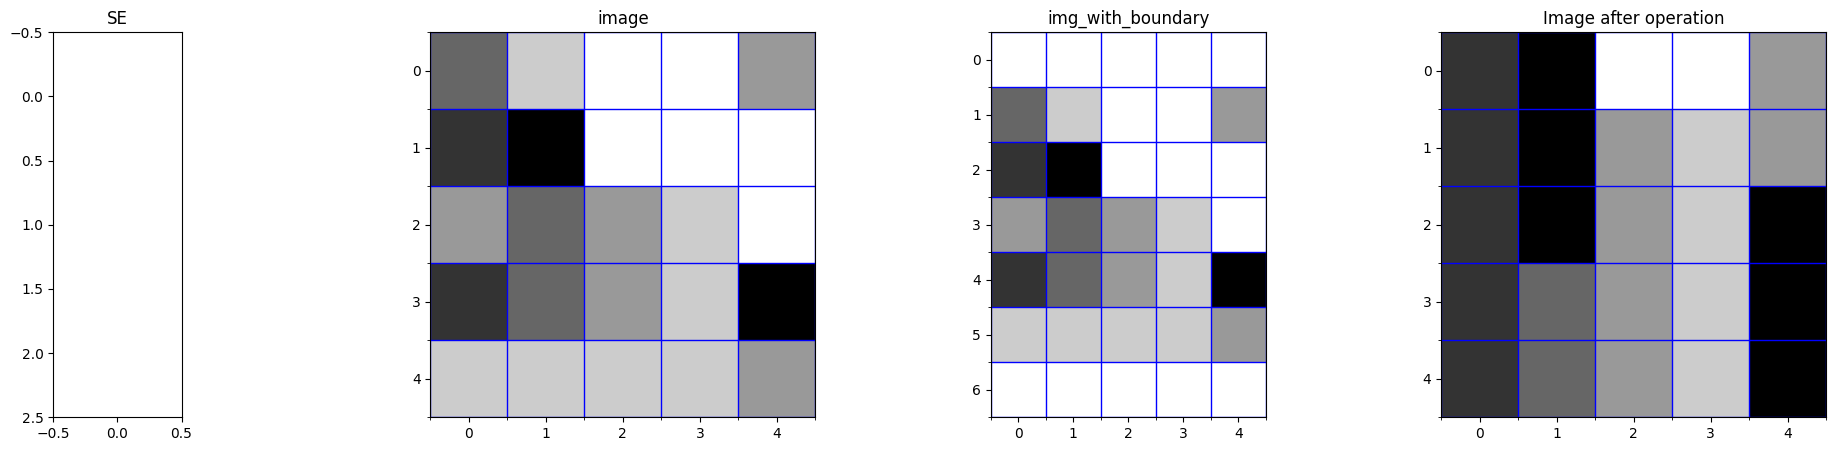
\includegraphics[width=\linewidth]{images/ef2_e2.png}
\caption{Erosion of f2 by vertical line of length 3}
\label{fig:ef2_e2}
\end{figure}
\\

\subsection{Erosion of f3 by horizontal line of length 3}
The center of this horizontal line SE would also be the middle pixel. The left and right border paddings of size 1 with the maximum value inside f3 are applied as indicated below as 'img\_with\_boundary' of Figure \ref{fig:ef3_e2}. In this task, each cell of f3 will be replaced by the minimum cell value among 3 cells in total which are overlapped with 1s from the SE. The final result is as shown in 'image after operation' of Figure \ref{fig:ef3_e2}.\\
\begin{figure}[h!]
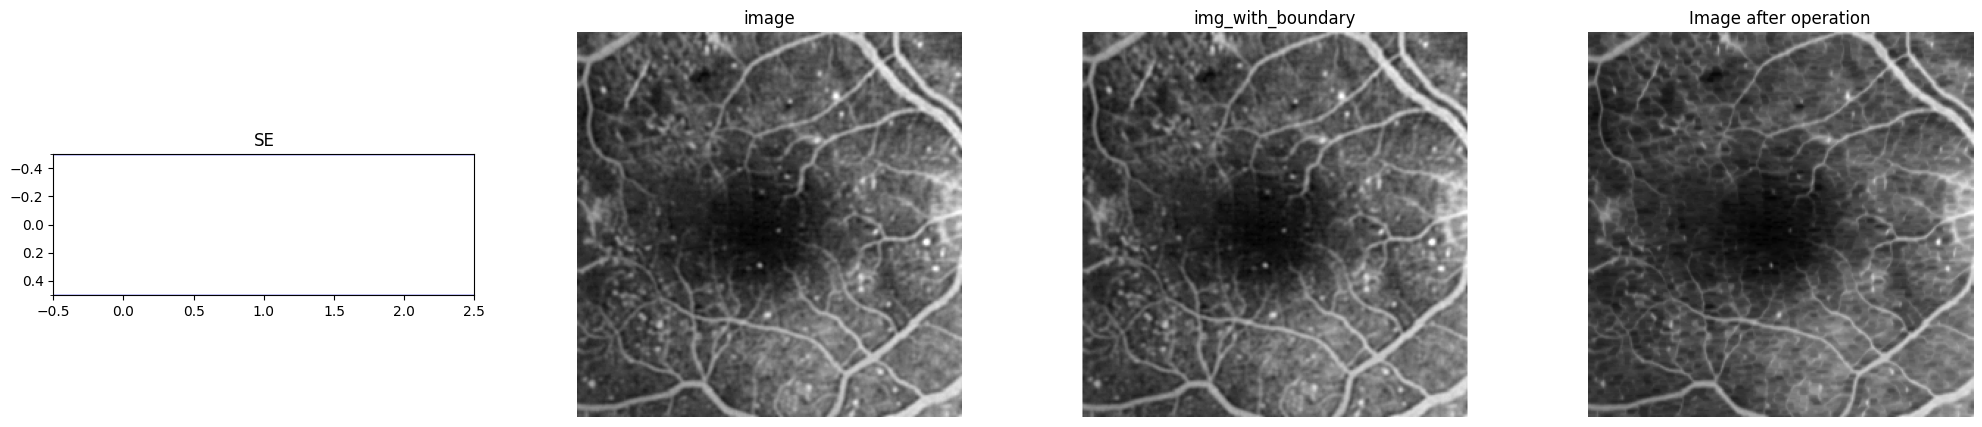
\includegraphics[width=\linewidth]{images/ef3_e2.png}
\caption{Erosion of f3 by horizontal line of length 3}
\label{fig:ef3_e2}
\end{figure}
\\ 

\subsection{Erosion of f3 by square of size 5}
The center(origin) of this SE would be the middle pixel. Since there are two rows and columns around the SE's center, border paddings of size 2 are added to f3, with the maximum pixel value of f3, as indicated below in 'img\_with\_boundary' of Figure \ref{fig:ef3_e3}. In this task, each cell of f3 will be replaced by the minimum cell value among 25 cells in total which are overlapped with 1s from the SE in each step. The final erosion result is as shown in 'image after operation' of Figure \ref{fig:ef3_e3}.\\
\begin{figure}[h!]
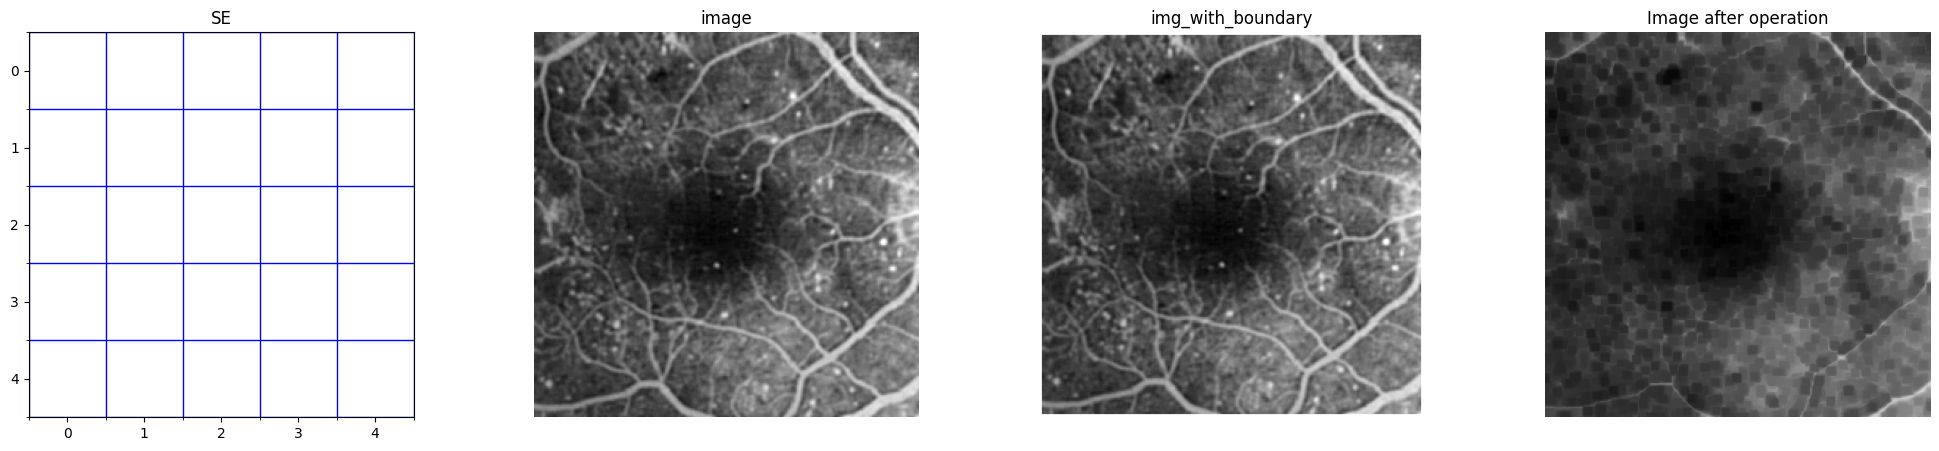
\includegraphics[width=\linewidth]{images/ef3_e3.png}
\caption{Erosion of f3 by square of size 5}
\label{fig:ef3_e3}
\end{figure}
\\
\newpage

\subsection{Erosion of f3 by backward diagonal (\textbackslash) of length 9}
The center of the SE would be the middle point. Since there are 4 more cells up and down around the SE's center, border paddings of size 4 are added to f3, with the maximum pixel value of f3, as indicated in 'img\_with\_boundary' of Figure \ref{fig:ef3_e4}. In this task, each cell of f3 will be replaced by the minimum cell value among 9 cells which are overlapped with 1s from the SE during each step. The final erosion result is as shown in 'image after operation' of Figure \ref{fig:ef3_e4}.\\
\begin{figure}[h!]
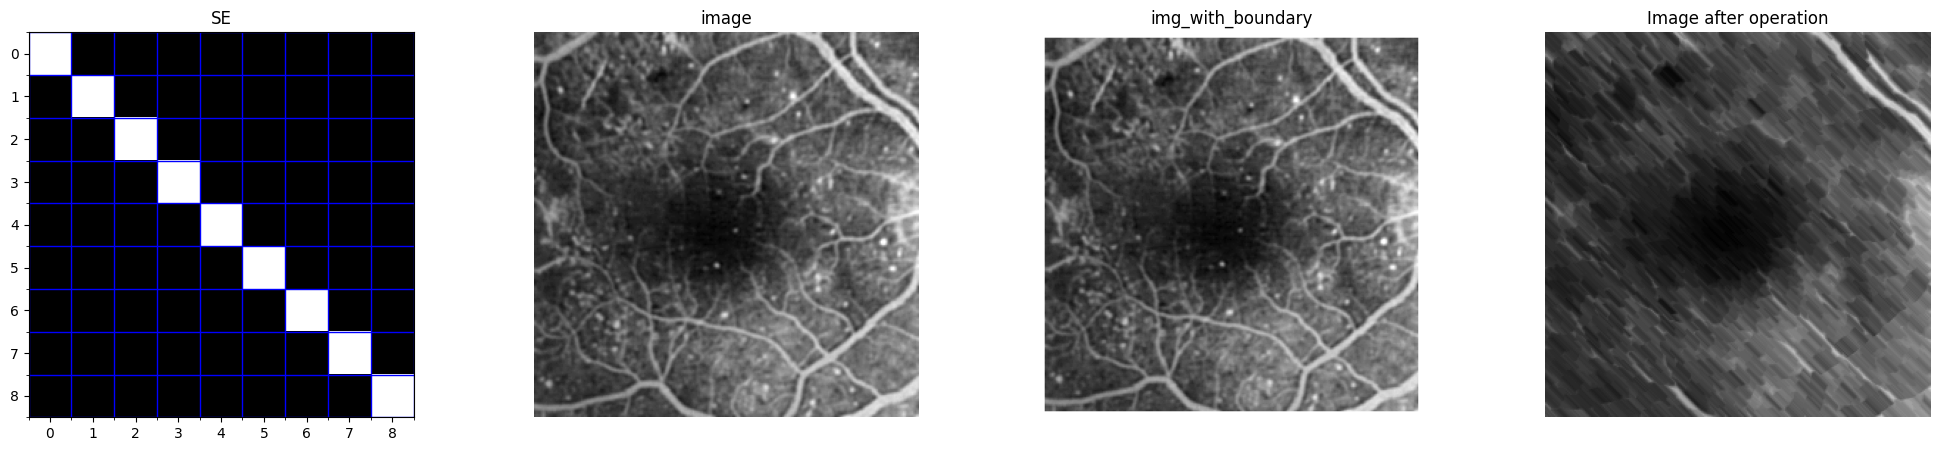
\includegraphics[width=\linewidth]{images/ef3_e4.png}
\caption{Erosion of f3 by backward diagonal (\textbackslash) of length 9}
\label{fig:ef3_e4}
\end{figure}
\\ 


\subsection{Erosion of f3 by forward diagonal (/) of length 9}
The center of the SE would be the middle point. Since there are 4 more cells up and down around the SE's center, border paddings of size 4 are added to f3, with the maximum pixel value of f3,as shown in 'img\_with\_boundary' of Figure \ref{fig:ef3_e5}. In this task, each cell of f3 will be replaced by the minimum cell value among 9 cells which are overlapped with 1s from the SE. The final erosion result is as shown in 'image after operation' in Figure \ref{fig:ef3_e5}.\\
\begin{figure}[h!]
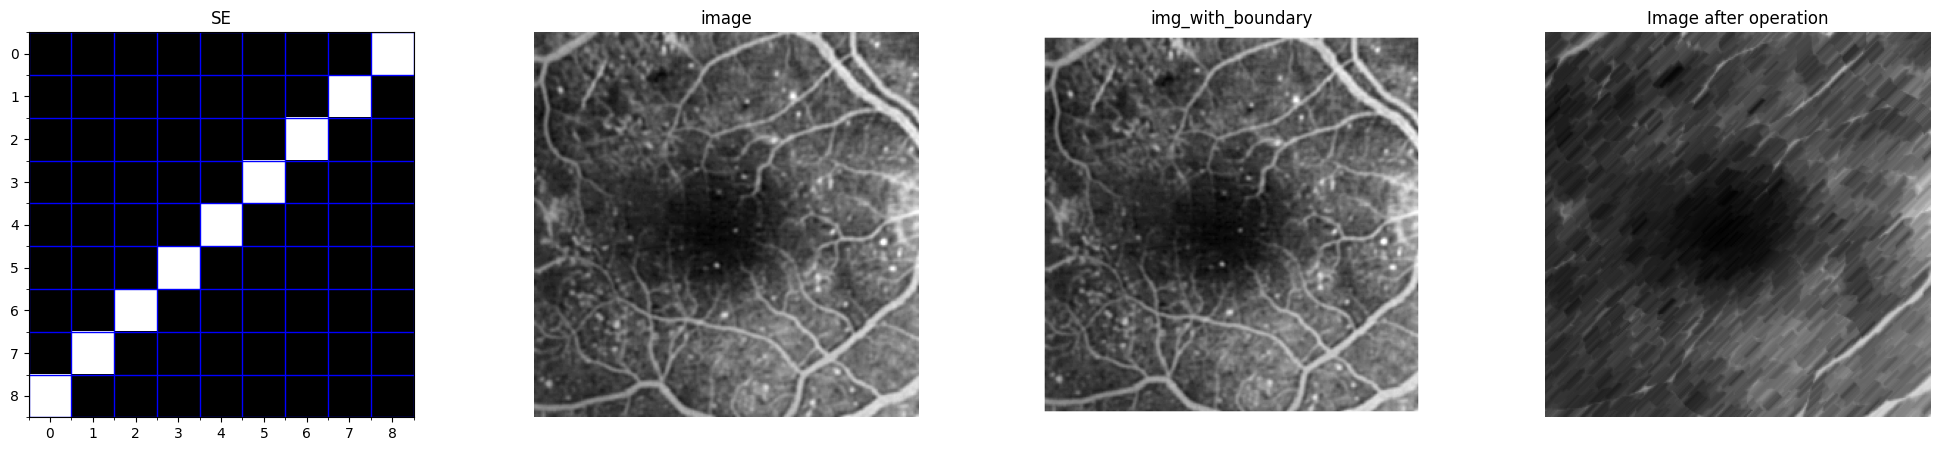
\includegraphics[width=\linewidth]{images/ef3_e5.png}
\caption{Erosion of f3 by forward diagonal (/) of length 9}
\label{fig:ef3_e5}
\end{figure}
\\

\section{Dilation}
During dilation, each cell value of the input image f3 will be replaced with the maximum value of the area where the SE matrix is overlapped during the iteration. \\
\subsection{Dilation of f3 by square of size 5}
The f3 image is padded with size 2, with 0 in each padded cell as shown in 'img\_with\_boundary'. During dilation, each cell value is replaced by the maximum value among 25 cells where all 1s from square-5 SE is being overlapped in each step. The final dilation result is as shown in 'image after operation' in Figure \ref{fig:df3_d3}.\\
\begin{figure}[h!]
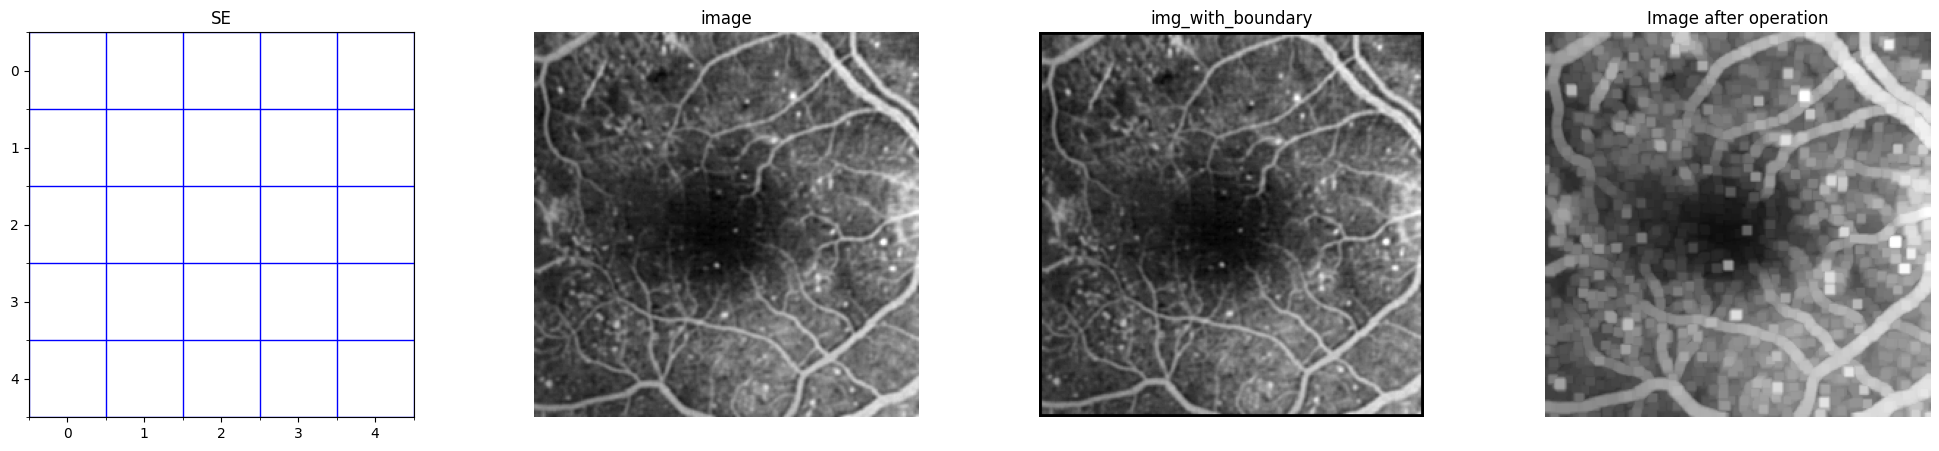
\includegraphics[width=\linewidth]{images/df3_d3.png}
\caption{Dilation of f3 by square of size 5}
\label{fig:df3_d3}
\end{figure}
\\ 

\subsection{Dilation of f3 by backward diagonal of length 9}
The f3 image is padded with size 4, with 0 in each padded cell as shown in 'img\_with\_boundary'. During dilation, each cell value is replaced by the maximum value among 9 cells where all 1s backward diagonal SE are being overlapped in each iteration step. The final dilation result is as shown in 'image after operation' in Figure \ref{fig:df3_d4}.\\
\begin{figure}[h!]
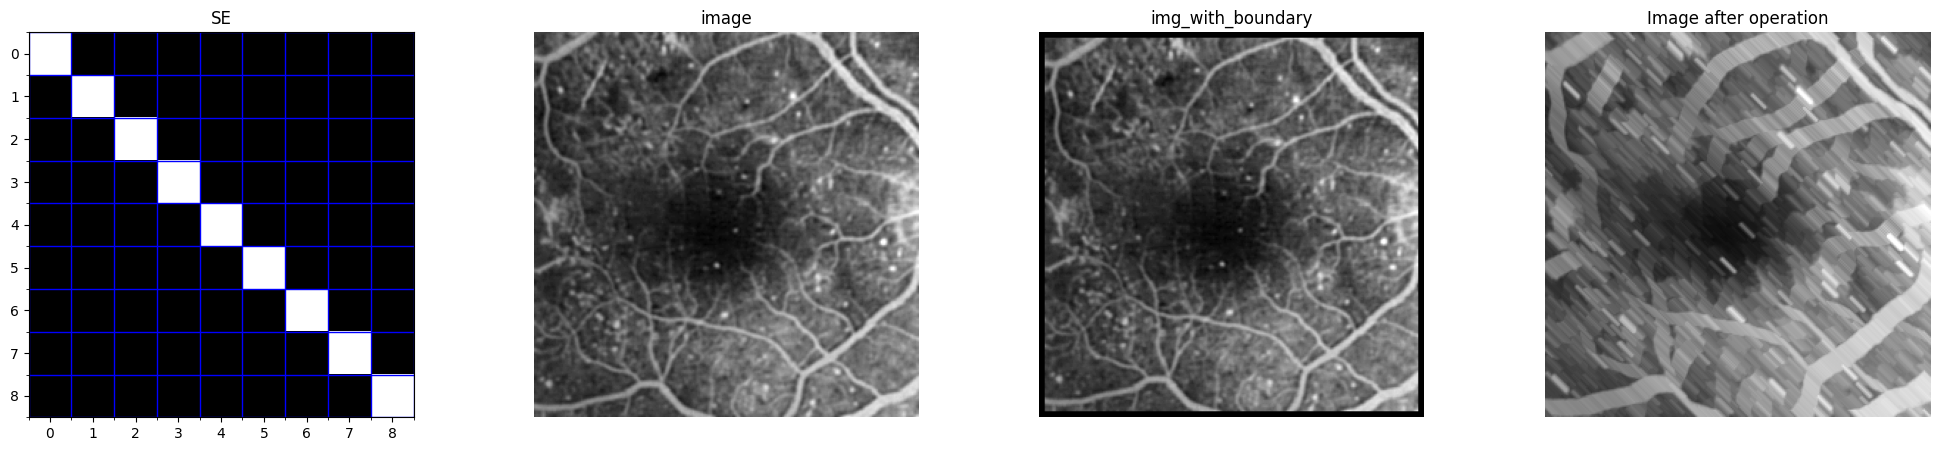
\includegraphics[width=\linewidth]{images/df3_d4.png}
\caption{Dilation of f3 by backward diagonal of length 9}
\label{fig:df3_d4}
\end{figure}
\\ 

\subsection{Dilation of f3 by forward diagonal of length 9}
The f3 image is padded with size 4, with value 0 in each padded cell as shown in 'img\_with\_boundary'. During dilation, each cell value is replaced by the maximum value among 9 cells where all 1s in the forward diagonal SE is being overlapped in each iteration step. The final dilation result is as shown in 'image after operation' in Figure \ref{fig:df3_d5}.\\
\begin{figure}[h!]
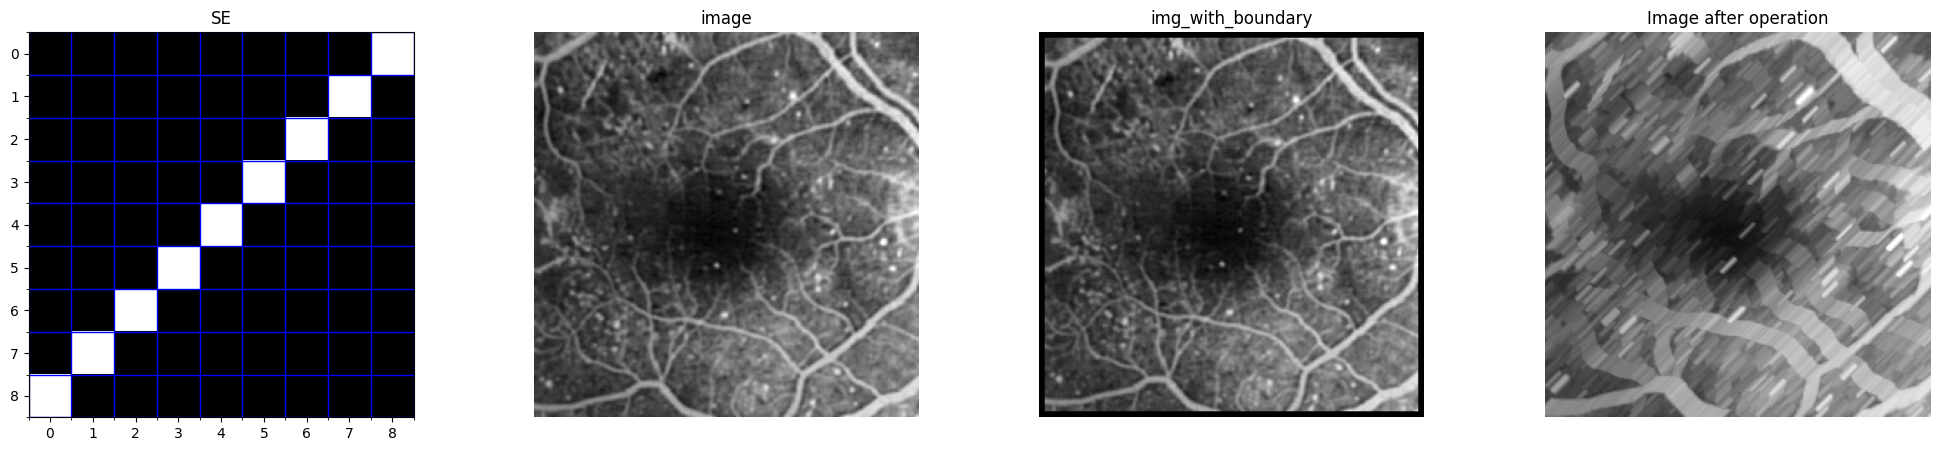
\includegraphics[width=\linewidth]{images/df3_d5.png}
\caption{Dilation of f3 by forward diagonal of length 9}
\label{fig:df3_d5}
\end{figure}
\\ 

\subsection{Dilation of "ef3\_e3.txt" by square of size 5}
The opening of the image is performing the dilation by using the point-reflected SE on the eroded image. Since the point-reflection of the square-5 SE is the same as the original square-5 SE, we can get the opening of f3 by performing dilation on the eroded image in the previous erosion task. \\
The eroded image 'ef3\_e3' is padded in all borders by size 2, where each cell value is 0. Then,  each cell value is replaced by the maximum value among 25 cells where all 1s in the square-5 SE is being overlapped in each step. The final dilation result is as shown in 'image after operation' in Figure \ref{fig:of3_o3}.\\
\begin{figure}[h!]
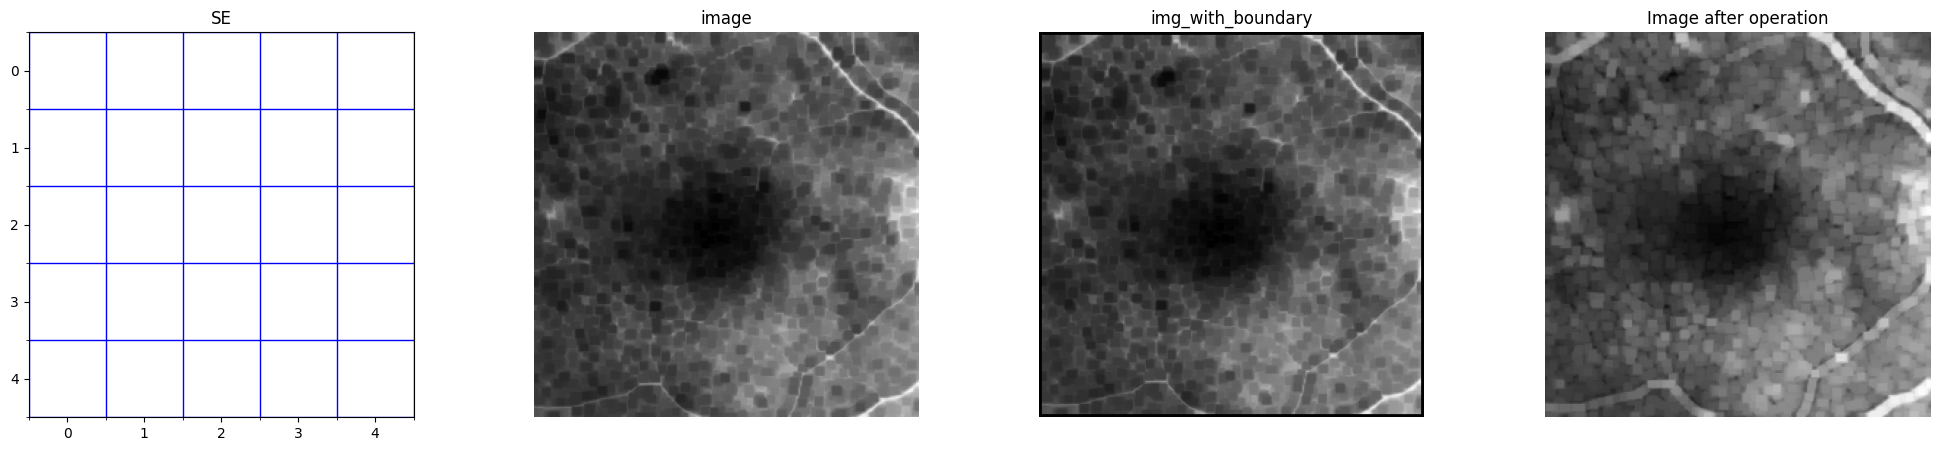
\includegraphics[width=\linewidth]{images/of3_o3.png}
\caption{Dilation of "ef3\_e3.txt" by square of size 5}
\label{fig:of3_o3}
\end{figure}
\\ 

\subsection{Dilation of "ef3\_e4.txt" by backward diagonal of length 9}
Since the point-reflection of the backward diagonal-9 SE is the same as the original backward diagonal-9 SE, we can get the opening of f3 by performing dilation on the eroded image in the previous erosion task. \\
The eroded image 'ef3\_e4' is padded in all borders by size 4, where each cell value is 0. Then, each cell value is replaced by the maximum value among 9 cells where all 1s in the backward diagonal-9 SE is being overlapped in each step. The final dilation result is as shown in 'image after operation' in Figure \ref{fig:of3_o4}.\\
\begin{figure}[h!]
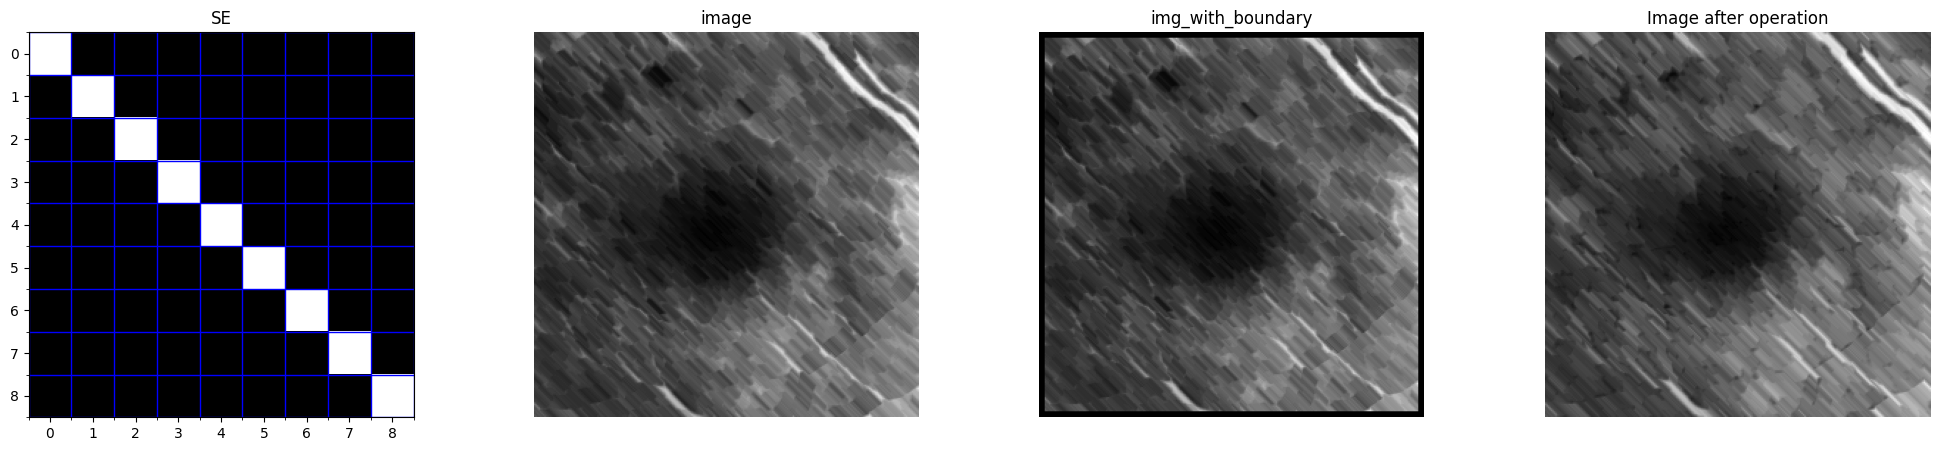
\includegraphics[width=\linewidth]{images/of3_o4.png}
\caption{Dilation of "ef3\_e4.txt" by backward diagonal of length 9}
\label{fig:of3_o4}
\end{figure}
\\ 
\newpage
\section{Self Implementation}
\subsection{One self-chosen experiment with an asymmetric SE not containing the center}
\begin{figure}[h!]
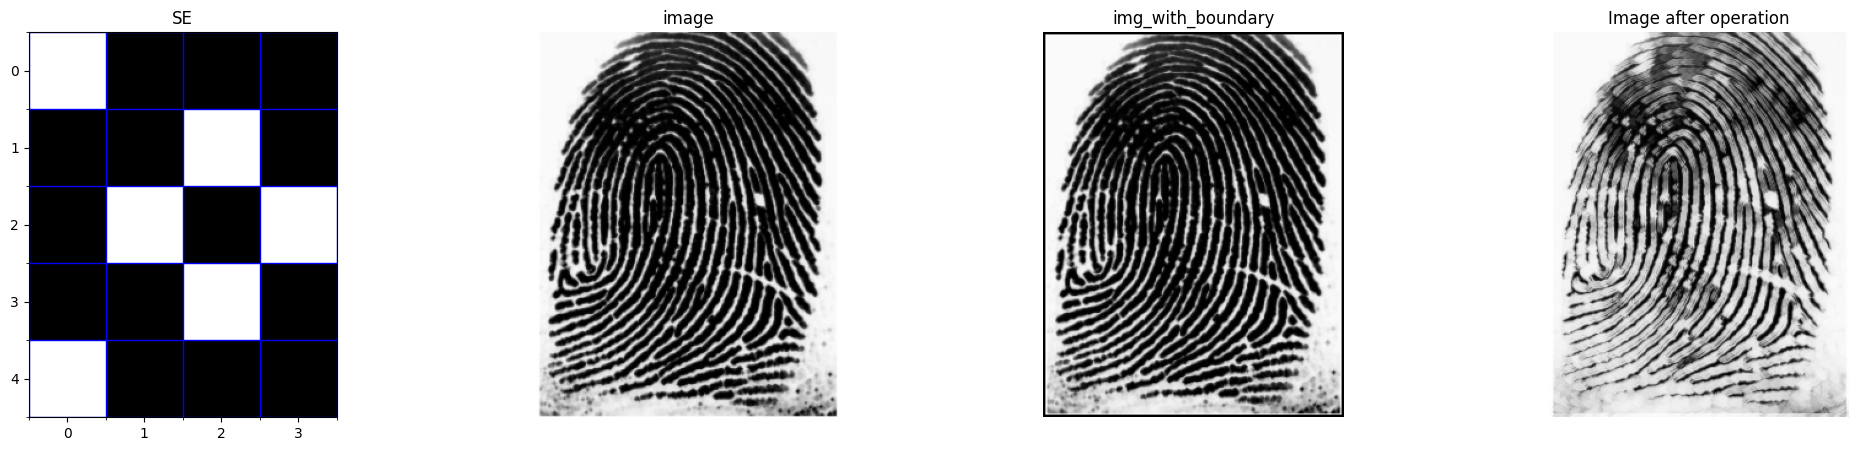
\includegraphics[width=\linewidth]{images/fingerprint-output.png}
\caption{Dilation of a fingerprint image with a asymmetric SE}
\label{fig:fingerprint}
\end{figure}
\\
\subsection{At least three self-chosen images and experiments}
\subsubsection{Image 1}
An image with corona virus is chosen as the first image to observe the virus’s outer crown via dilation. The size of SE is 5, so the wolf image is bordered with padding size 2, where the values of those border cells are 0. This bordered image can be seen as 'img\_with\_boundary' in Figure \ref{fig:corona}. \\
The center point of the SE is the origin. During this dilation, each cell of the corona image will be replaced by the maximum cell value among 25 cells which are overlapped with 1s from the SE. The final dilation result is as shown in 'image after operation' of Figure \ref{fig:corona}.\\
\begin{figure}[h!]
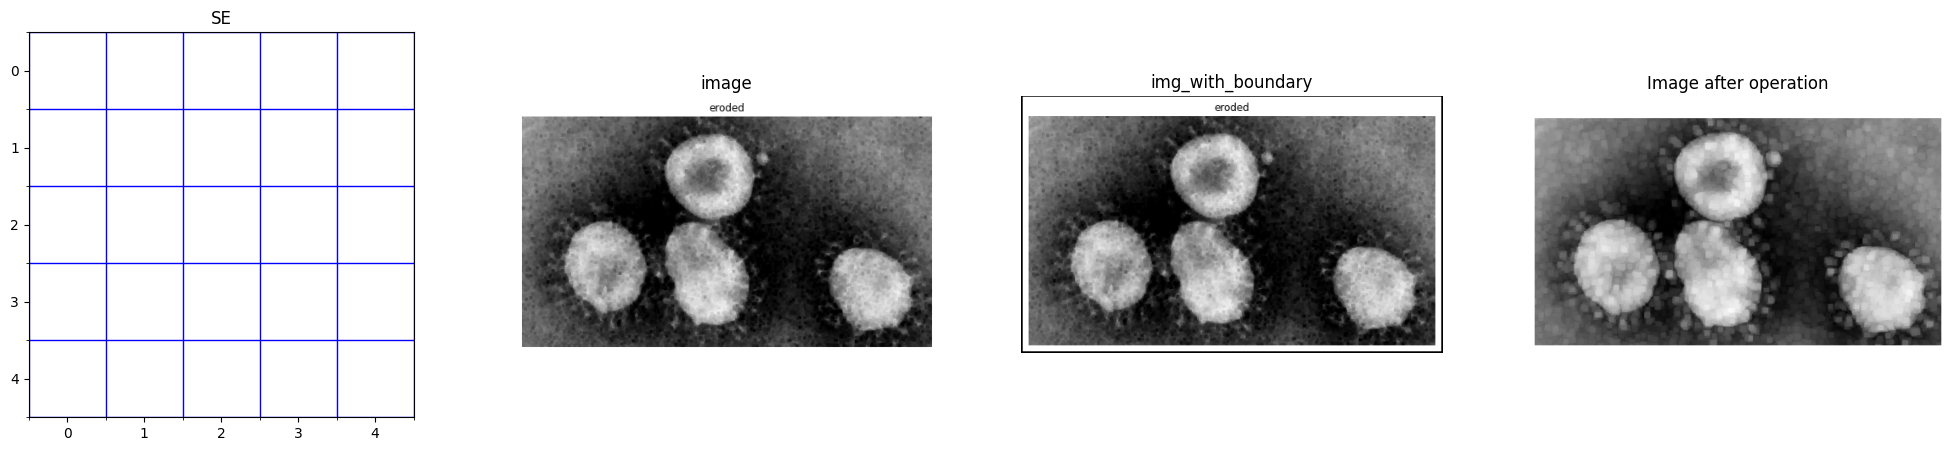
\includegraphics[width=\linewidth]{images/corona_output.png}
\caption{Dilation of a corona image to observe the virus's outer crown}
\label{fig:corona}
\end{figure}
\\ 

\subsubsection{Image 2}
A wolf image is chosen to make the furs of the wolf thinner via erosion. The size of SE is 3, so the wolf image is bordered with padding size 1, where the values of those border cells are 255. This bordered image can be seen as 'img\_with\_boundary' in Figure \ref{fig:wolf}. \\
The ones in the SE are being placed as a \textbf{'+'} symbol, where the center point is the origin as usual. During this erosion, each cell of the wolf will be replaced by the minimum cell value among 5 cells which are overlapped with 1s from the SE. The final erosion result is as shown in 'image after operation' of Figure \ref{fig:wolf}.\\
\begin{figure}[h!]
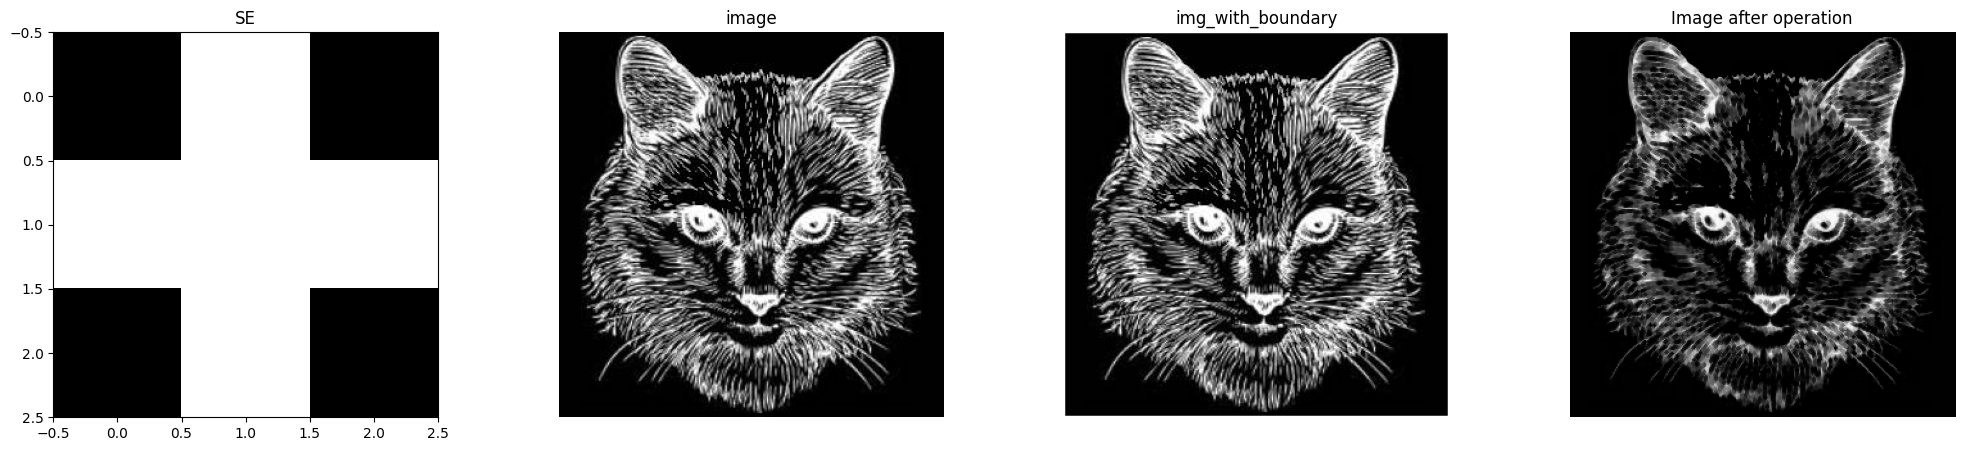
\includegraphics[width=\linewidth]{images/wolf.png}
\caption{Erosion of a wolf image with a plus-shaped SE of size 3}
\label{fig:wolf}
\end{figure}
\\ 

\subsubsection{Image 3}
An image with roots is chosen as the last image to make the roots thicker via dilation. The SE is chosen to be filled with ones which are the remaining cells of a outer \textbf{'+'}shape. The size of SE is 4, so the root image is bordered with padding size 2, where the values of those border cells are 0. This bordered image can be seen as 'img\_with\_boundary' in Figure \ref{fig:roots}. \\
The center point of the SE will the origin. During this dilation, each pixel value of the root image will be replaced by the maximum cell value among 8 cells which are overlapped with 1s from the SE in each step. The final dilation result is as shown in 'image after operation' of Figure \ref{fig:roots}.\\
\begin{figure}[h!]
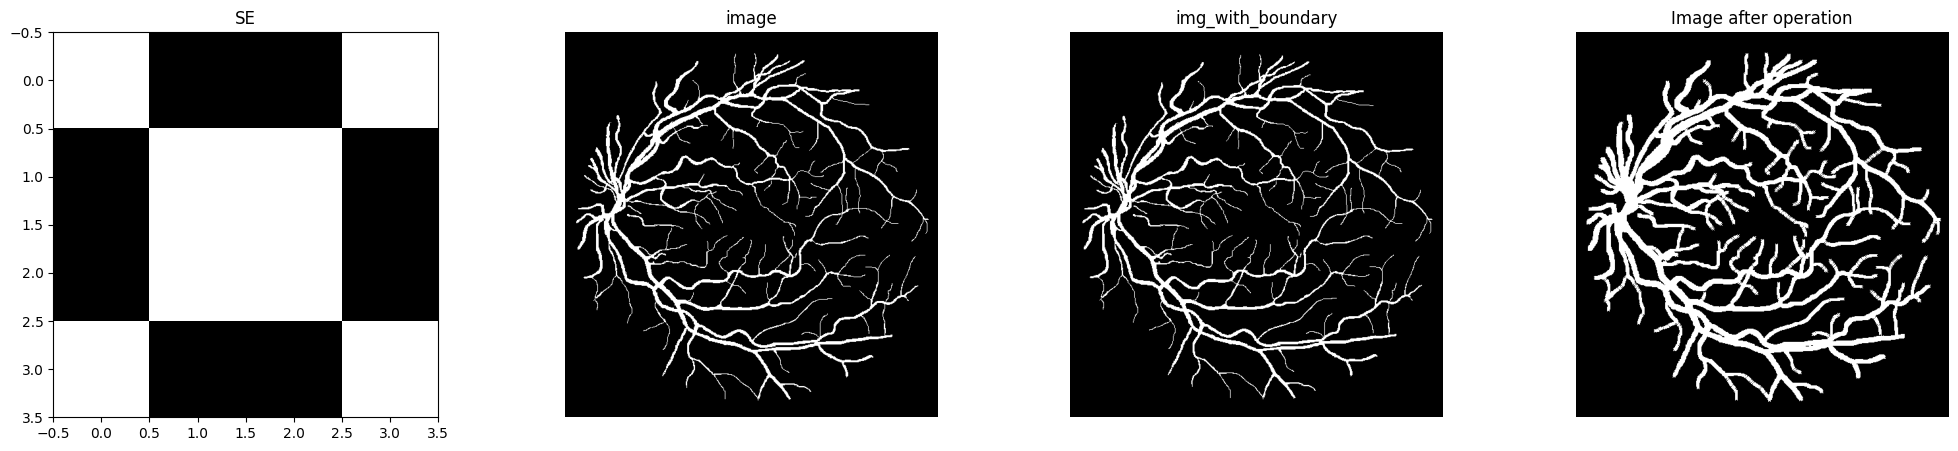
\includegraphics[width=\linewidth]{images/roots_dilated.png}
\caption{Dilation of image with roots}
\label{fig:roots}
\end{figure}
\\
\subsection{Other experiments with morphological operations on images}
\begin{figure}[h!]
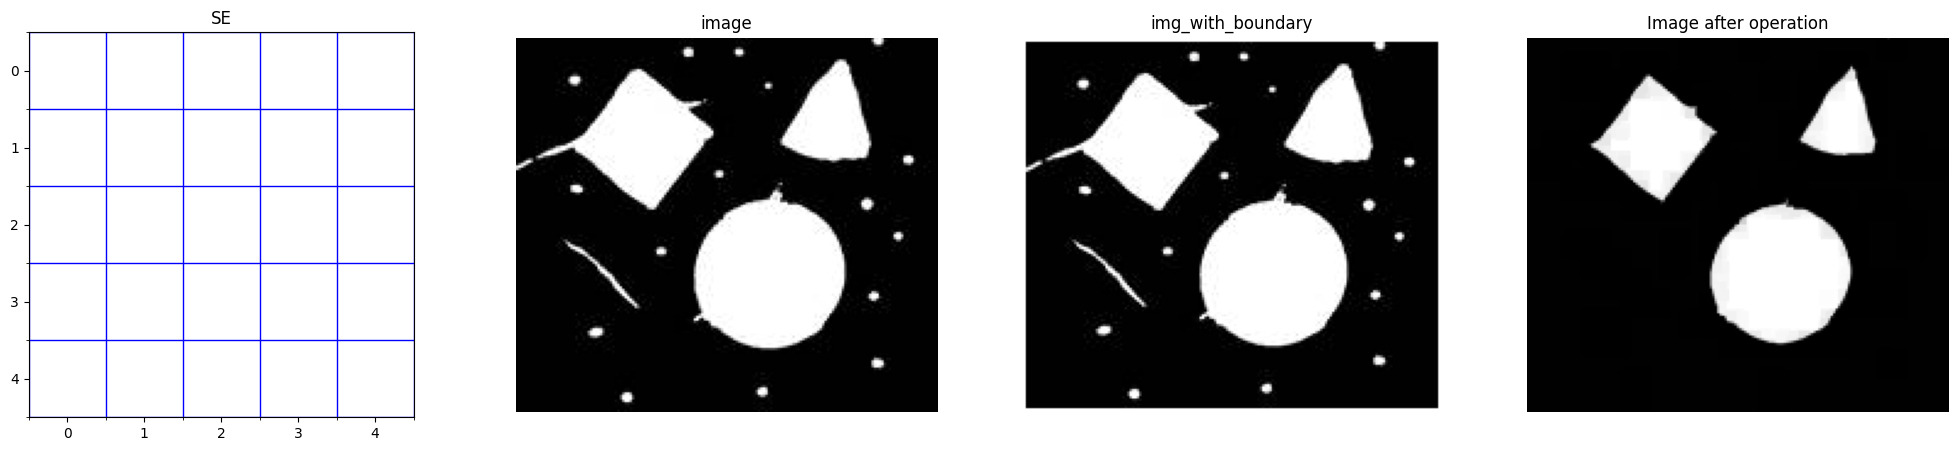
\includegraphics[width=\linewidth]{images/sample_img1.png}
\caption{Erosion of image with shapes and background noise}
\label{fig:sample_1}
\end{figure}
\begin{figure}[h!]
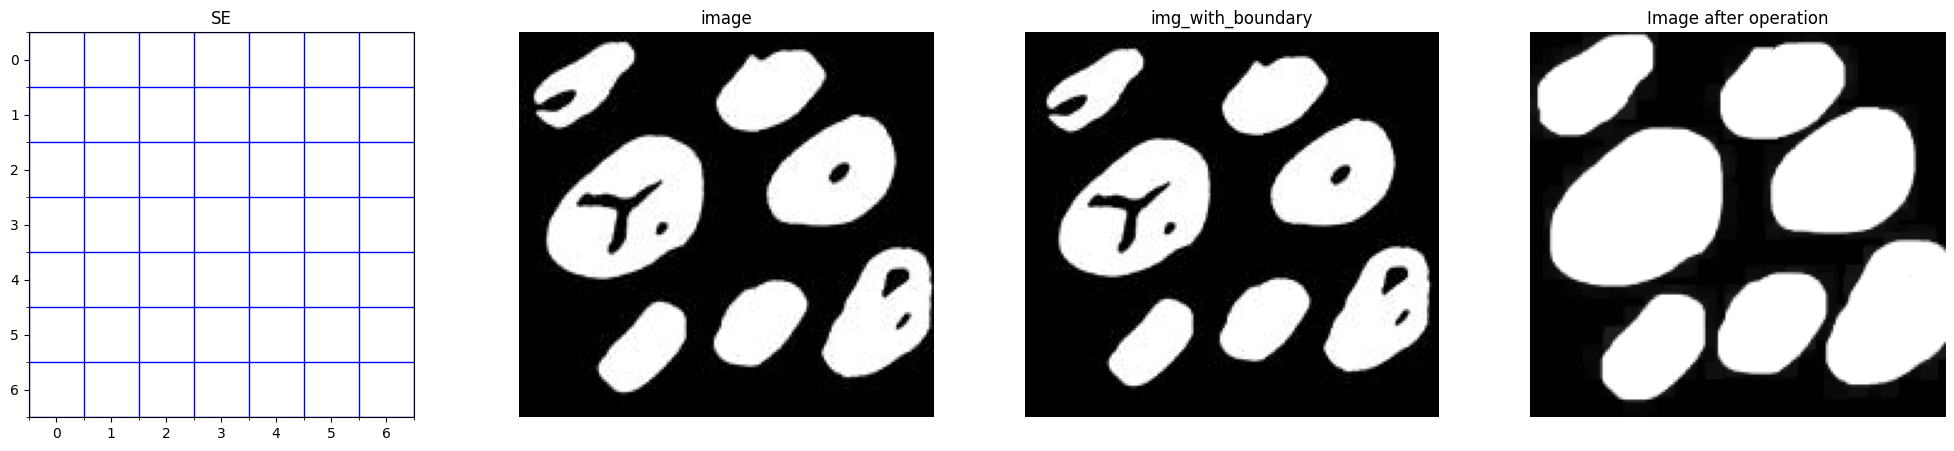
\includegraphics[width=\linewidth]{images/sample_img2.png}
\caption{Dilation of image with shapes}
\label{fig:sample_2}
\end{figure}
\begin{figure}[h!]
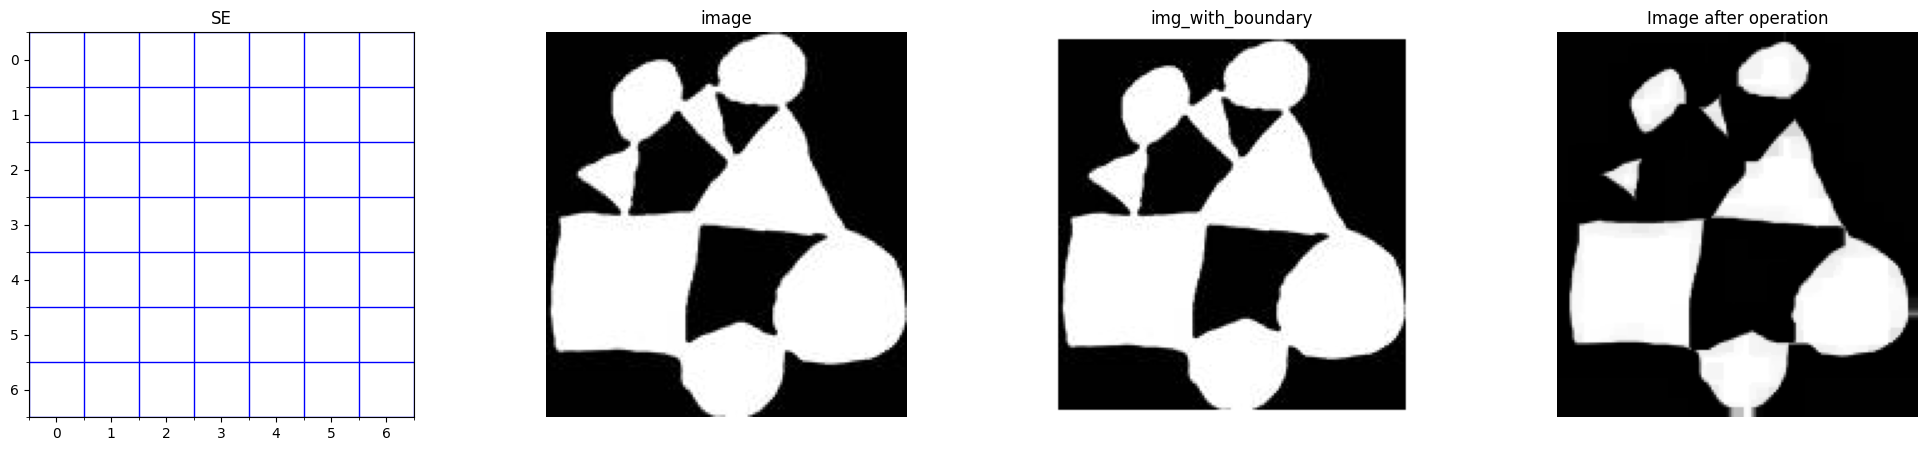
\includegraphics[width=\linewidth]{images/sample_img3.png}
\caption{Erosion of image with connected shapes for shape separate }
\label{fig:sample_3}
\end{figure}

\begin{thebibliography}{9}

\bibitem{corona-image} 
\text{Corona Image}. 
\url{https://www.dw.com/image/51961691\_401.jpg}

\bibitem{cat} 
\text{cat-image.}\url{https://www.vectorstock.com/royalty-free-vector/hand-drawn-portrait-cute-cat-sketch-art-vector-13666593}
\bibitem{cnn} 
\text{T. A. Soomro et al., "Impact of Image Enhancement Technique on CNN Model for Retinal Blood Vessels Segmentation," in IEEE Access, vol. 7, pp. 158183-158197, 2019, doi: \url{10.1109/ACCESS.2019.2950228}}

\bibitem{random} 
\text{Images with shapes.}\url{http://what-when-how.com/introduction-to-video-and-image-processing/morphology-introduction-to-video-and-image-processing-part-1/}

\bibitem{} 
\text{Nickson Joram}
\textit{Morphological Operations in Image Processing}
\url{https://himnickson.medium.com/morphological-operations-in-image-processing-cb8045b98fcc}


\end{thebibliography}


\end{document}

